\section{Mealy machines with timers}

\subsection{Definition and timed semantics}
We assume an infinite set $X = \{ x_1, x_2, x_3,\ldots \}$ of {\em timers}.
Let $\toevents$ be the set of {\em timeout events} of the form
$\toevent{x}$ for $x \in X$.
For a set $I$, let $\extinputs$ be $I \cup \toevents$.
%
We write $A \hookrightarrow B$ for the set of partial functions from $A$ to $B$.
With $f \lceil A$ we denote the restriction of function $f$ to $\domof{f} \cap A$.
%For arbitrary functions $f$ and $g$, $f [g]$ is the function with domain $\domof{f}$ that behaves like $f$
%on $\domof{f} \setminus \domof{g}$ and like $g$ on $\domof{f} \cap \domof{g}$.
We write $\finitesubsets{A}$ for the set of finite subsets of set $A$.

\begin{definition}
\label{def:MMT}
A \emph{Mealy machine with timers (MMT)} is a tuple
\\
$\M = (I, O, Q, q_0, \vars, \delta, \lambda, \remap)$, where
\begin{itemize}
\item
$I$ and $O$ are finite sets of input events and output events, respectively,
\item
$Q$ is a finite set of states,
with
$q_0 \in Q$ the initial state,
\item
$\vars: Q \rightarrow \finitesubsets{X}$, with $\varsof{q_0} = \emptyset$,
\item
$\delta: Q \times \extinputs \hookrightarrow  Q$ is a transition function,
%with $\delta(q,i)$ defined iff $q \in Q$ and $i \in I \cup \{ \toevent{x} \mid x \in \varsof{q} \}$, 
\item
$\lambda: Q \times \extinputs \hookrightarrow O$ is an output function, 
\item
$\remap : Q \times \extinputs \hookrightarrow (X \hookrightarrow \natplus)$ is a timer update function.
\end{itemize}
Let $q \in Q$, $i \in \extinputs$, $q'=\delta(q,i)$ and $\rho=\remap(q,i)$. 
We require that $\varsof{q'} \setminus \varsof{q} \subseteq \domof{\rho} \subseteq\varsof{q'}$. 
When timer $x$ expires it is either stopped or restarted:
if $i=\toevent{x}$, for some $x$, then $x \not\in \varsof{q'} \setminus \domof{\rho}$.
%
We also require that input events are always enabled and timeout events are enabled
for timers that are active in the current state:
$\delta(q,i)$, $\lambda(q,i)$ and $\pi(q,i)$ are defined iff either
$i \in I$ or $i=\toevent{x}$, for some $x \in\varsof{q}$.
We write $q \xrightarrow{i/o,\rho} q'$ if $\delta(q,i) = q'$, $\lambda(q,i)= o$ and $\remap(q,i) = \rho$.
\end{definition}
Update function $\remap$ determines how timers are affected when an event occurs.
Basically, four things may happen.
%\marginpar{Add Venn diagram to illustrate situation?}
Let $q \in Q$, $i \in \extinputs$, $\delta(q,i)=q'$ and $\remap(q,i)=\rho$.
\begin{enumerate}
\item
If $x \in\varsof{q} \setminus \varsof{q'}$ then input $i$ \emph{stops} timer $x$.
\item
If $x \in \varsof{q'} \setminus \varsof{q}$ then $i$ \emph{starts} timer $x$ with value $\rho(x)$.
\item
If $x \in \varsof{q} \cap \domof{\rho}$ then $i$ \emph{restarts} timer $x$ with value $\rho(x)$.
\item
Finally, if $x \in \varsof{q'} \setminus \domof{\rho}$ then timer $x$ is \emph{unaffected} by $i$.
\end{enumerate}

\paragraph{Semantics.}
The semantics of MMT $\M = (I, O, Q, q_0, \vars, \delta, \lambda, \remap)$ is defined via an infinite state transition system that describes all possible
configurations and transitions between them.
A \emph{valuation} is a partial function
$\tvals : X \hookrightarrow \realsplus$, defined on a finite subset of $X$, that assigns nonnegative real numbers as values to timers.
We write $\Vals{Y}$ for the set of valuations with domain $Y \subseteq X$.
A \emph{configuration} of an MMT is a pair $(q,\tvals)$, where $q \in Q$ is a state and $\tvals\in\Vals{\varsof{q}}$ is a valuation.
The \emph{initial configuration} is the pair $(q_0, \tvals_0)$, where $\tvals_0$ is the empty function.
Valuations and configurations can be modified by the occurrence of input and timeout events, and by
the occurrence of delays.
If $\tvals$ is a valuation in which all timers
have a value of at least $d$, then $d$ units of time may pass. As a result of this delay the value of all the timers is decremented by $d$.
Formally, for $\tvals, \tvals'$ valuations and $d \in \delays$, we define a delay transition relation by
\begin{eqnarray*}
\tvals \xrightarrow{d} \tvals' & \Leftrightarrow & [\domof{\tvals} = \domof{\tvals'} \wedge \forall x \in\domof{\tvals} : \tvals'(x) = \tvals(x) - d ].
\end{eqnarray*}
If the current valuation is $\tvals$, then timeout event $\toevent{x}$ may occur only if $\tvals(x)=0$.
If an input or a timeout event occurs, $\tvals$ is updated as specified by update function $\rho$.
The values of timers that are not affected by $\rho$ remain unchanged.
Formally, for $\tvals, \tvals'$ valuations, $i \in \extinputs$, $o \in O$ and $\rho \in X \hookrightarrow \natplus$,
we define a discrete transition relation by
\begin{eqnarray*}
\tvals \xrightarrow{i/o, \rho}  \tvals' & \Leftrightarrow & [ \domof{\tvals'} \setminus \domof{\tvals}  \subseteq \domof{\rho} \subseteq \domof{\tvals'} ~ \wedge\\
&& [\forall x \in\domof{\tvals'} : \tvals'(x) = \mbox{ if } x \in\domof{\rho} \mbox{ then } \rho(x) \mbox{ else } \tvals(x)] ~ \wedge\\
%More concise but harder to understand:
%&& \tvals' =  \tvals'[\tvals][\rho] ~ \wedge \\
&& \forall x \in X : i=\toevent{x} \Rightarrow (\tvals(x) = 0 \wedge x \not\in\domof{\tvals'} \setminus \domof{\rho})].
\end{eqnarray*}
%Condition $\tvals' =  \tvals'[\tvals][\rho]$ expresses that $\tvals'$ is obtained by giving variables
%in $\domof{\rho}$ the value specified by $\rho$, and all remaining variables the value specified by $\tvals$.
Transition relations $\xrightarrow{d}$ and $\xrightarrow{i/o, \rho}$ can be easily lifted to configurations.
For all configurations $(q, \tvals)$, $(q', \tvals')$ of an MMT $\M$,
\[
\frac{q = q' \quad \tvals \xrightarrow{d} \tvals'}{(q,\tvals) \xrightarrow{d} (q',\tvals')}
\quad\quad
  \frac{q \xrightarrow{i/o,\remapinst} q' \quad \tvals \xrightarrow{i/o, \rho} \tvals'}{(q,\tvals) \xrightarrow{i/o} (q',\tvals')}
\]
A \emph{timed run} of $\M$ over $w$ is a sequence 
\begin{eqnarray*}
\alpha & = & C_0 \xrightarrow{d_1} C'_0 \xrightarrow{i_1/o_1} C_1 \xrightarrow{d_2} C'_1 \xrightarrow{i_2/o_2} C_2 \cdots
\xrightarrow{d_k} C'_{k-1} \xrightarrow{i_k/o_k} C_{k}
\end{eqnarray*}
of transitions between configurations $C_j, C'_j$ of $\M$, where $C_0$ is the initial configuration.
%Note that, since MMTs are deterministic (if we allow to observe the
%identities of timers in timeout events),
%for each timed word $w$ there exists at most one run over $w$.
A \emph{timed word} over inputs $I$ and outputs $O$ is a sequence
\begin{eqnarray*}
w & = &  d_1 ~ i_1 ~ o_1 ~ d_2 ~ i_2 ~ o_2 \cdots d_k ~ i_k ~ o_k,
\end{eqnarray*}
where $d_j \in \delays$, $i_j \in I \cup \{ \mathit{to} \}$, and $o_j \in O$.
To each timed run $\alpha$ we associate a \emph{timed word} by forgetting the configurations and the timers
in timeout events:
\begin{eqnarray*}
\timedword(\alpha) & = & d_1 ~ i'_1 ~ o_1 ~ d_2 ~ i'_2 ~ o_2 \cdots d_k ~ i'_k ~ o_k, \mbox{ where for all } j,
i'_j  =  \left\{ \begin{array}{ll}
i_j & \mbox{if } i_j \in I,\\
\mathit{to} & \mbox{if } i_j \in \toevents.
\end{array} \right.
\end{eqnarray*}
The idea is that timeouts cannot be observed directly. 
However, when we observe an output that is not triggered by an input, we may
conclude that a timeout occurred. But in general we do not know which timer expired.

We say $w$ is a timed word of $\M$ if $\M$ has a timed run $\alpha$ with $w = \timedword(\alpha)$.
%
Two MMTs $\M$ and $\N$ with the same sets of inputs are \emph{timed equivalent}, denoted $\M \approx_{\mathit{timed}} \N$, iff 
they have the same sets of timed words.

\iflong
\paragraph{Remark.}
In our semantics we assume that discrete transitions occur instantaneously and take no time. In applications, however, i/o interactions
often take a significant amount of time. In \cite{SHV16}, for instance, a case study of an interventional X-ray system is
described in which a single i/o interaction may take several seconds. If it is important to model such delays
explicitly, this can be done within the MMT framework by splitting a transition with input $i$ and output $o$ into
a pair of consecutive transitions: a first transition with input $i$ and some default output $\Lambda$ that starts
a timer $x$, and a second transition in which $x$ times out and output $o$ is produced.
If inputs arrive in the newly introduced intermediate state, these may either be ignored, buffered or forbidden
(via a transition to some designated error state).
Note that $\Lambda$ corresponds to the \emph{absence} of an observable output. For inputs $i \in I$ this is fine: if such
an input does not trigger an observable output then we just assume that the output event is $\Lambda$. We do not allow
$\Lambda$ as output event in timeout transitions $\toevent{x}$: since timeout events themselves are not observable, we can ony observe their occurrence indirectly through the observable output that they trigger.

\paragraph{Remark.}
Note that we assume that in a timed run each discrete transition is preceded by a nonzero delay.
The idea that multiple consecutive discrete transitions may occur in zero time is a useful abstraction in synchronous
programming and in the theory of timed automata, but nonzero delays form
a crucial requirement for the learning algorithm that we present in this paper.

Disallowing zero delays creates certain complications that we have to deal with. The simple MMT of Figure~\ref{fig:timelock}, for instance,
may reach a timelock following the timed word $1 ~ i ~ o ~ 1 ~ i ~ o$: at this point timer $x$ has value $0$, but no timeout is enabled since first a nonzero amount of time has to elapse, which is not possible since then $x$ would become negative.
\begin{figure}[ht]
\begin{center}
\begin{tikzpicture}[->,>=stealth',shorten >=1pt,auto,node distance=2.5cm,main node/.style={circle,draw,font=\sffamily\large\bfseries}]
  \node[initial, state] (1) {$q_0$};
  \node[state] (2) [right of=1] {$q_1$};
  \node[state] (3) [right of=2] {$q_2$};
  
  \path[every node/.style={font=\sffamily\scriptsize}]
    (1) edge node {$i/o$, $~x:=1$} (2)  
    (2) edge  node {$\toevent{x}/o'$} (3)
        edge  [loop below] node {$i/o$} (2)
    (3) edge  [loop below] node {$i/o$} (4);
\end{tikzpicture}
\caption{An MMT with a timelock}
\label{fig:timelock}
\end{center}
\end{figure}
Once solution would be to disable inputs in $I$ whenever a timer has become $0$. 
In Section~\ref{section untimed semantics}, we will elaborate
a different approach in which we only consider runs in which no ``races'' occur. This eliminates the problematic
behavior of the above MMT in which there is a race between the second $i$ event and the timeout.
\fi

\paragraph{Nondeterminism.}
Due to our assumption that we cannot observe the identity of a timer in a timeout event, an MMT may exhibit nondeterministic
behavior: even if we offer exactly the same inputs at exactly the same time, different outputs may occur in different runs. 
The MMT of Figure~\ref{fig:nondeterminism}, for instance, accepts both the timed words
$1 ~ i ~ o ~ 1 ~ \mathit{to} ~ o'$ and $1 ~ i ~ o ~ 1 ~ \mathit{to} ~ o''$.
(For clarity, we omit some self-loop transitions.)
\begin{figure}[ht]
\vspace{-2em}
\begin{center}
\begin{tikzpicture}[->,>=stealth',shorten >=1pt,auto,node distance=2.5cm,main node/.style={circle,draw,font=\sffamily\large\bfsthe name of the eries}]
  \node[initial, state] (1) {$q_0$};
  \node[state] (2) [below of=1] {$q_1$};
  \node[state] (3) [right of=2] {$q_3$};
  \node[state] (4) [left of=2] {$q_2$};

  \path[every node/.style={font=\sffamily\scriptsize}]
    (1) edge node {$i/o$, $~x:=1$, $y:=1$} (2)  
    (2) edge  node {$\toevent{x}/o'$} (3)
     edge  node {$\toevent{y}/o''$} (4);
\end{tikzpicture}
\caption{An MMT with nondeterministic behavior}
\label{fig:nondeterminism}
\end{center}
\end{figure}
\iflong
In order to rule out this type of nondeterminism, it is not enough to require that the timer update functions are injective,
that is, it is not allowed to assign the same value to multiple timers in a single transition.
This is illustrated by the MMT of Figure~\ref{fig:nondeterminism2}, which accepts both the timed words
$1 ~ i ~ o ~ 1 ~ \mathit{to} ~ o'~ 1 ~ \mathit{to} ~ o'$ and $1 ~ i ~ o ~ 1 ~ \mathit{to} ~ o' ~ 1 ~ \mathit{to} ~ o''$.
\begin{figure}[ht]
\begin{center}
\begin{tikzpicture}[->,>=stealth',shorten >=1pt,auto,node distance=2.5cm,main node/.style={circle,draw,font=\sffamily\large\bfseries}]
  \node[initial, state] (1) {$q_0$};
  \node[state] (2) [below of=1] {$q_1$};
  \node[state] (4) [left of=2] {$q_2$};

  \path[every node/.style={font=\sffamily\scriptsize}]
    (1) edge node {$i/o$, $~x:=1$, $y:=2$} (2)  
    (2) edge  node {$\toevent{y}/o''$} (4)
      edge  [loop right] node {$\toevent{x}/o'$, $~x:=1$} (2);
\end{tikzpicture}
\caption{Another MMT with nondeterministic behavior}
\label{fig:nondeterminism2}
\end{center}
\end{figure}
\fi
%
The nondeterminism of the MMTs of Figure~\ref{fig:nondeterminism} 
%and \ref{fig:nondeterminism2} 
is ``uncontrollable'' and occurs after any (nonempty) input sequence.
Figure~\ref{fig:nondeterminism3} gives an example of an MMT that exhibits nondeterminism when the second input occurs \emph{exactly} one time unit after the first input: the MMT accepts timed words
$7 ~ i ~ o ~ 1 ~ i ~ o ~ 1 ~ \mathit{to} ~ o'$ and $7 ~ i ~ o ~ 1 ~ i ~ o ~ 1 ~ \mathit{to} ~ o''$.
This type of nondeterminism is ``controllable'' and will not occur if we are careful
when selecting the timing of inputs.
\begin{figure}[ht]
\vspace{-2em}
\begin{center}
\begin{tikzpicture}[->,>=stealth',shorten >=1pt,auto,node distance=2.5cm,main node/.style={circle,draw,font=\sffamily\large\bfseries}]
  \node[initial, state] (1) {$q_0$};
  \node[state] (2) [right of=1] {$q_1$};
  \node[state] (3) [right of=2] {$q_2$};

  \path[every node/.style={font=\sffamily\scriptsize}]
    (1) edge node {$i/o$, $~x:=2$} (2)  
    (2) edge  node {$i/o$, $~y:=1$} (3)
      edge  [loop below] node {$\toevent{x}/o$, $~x:=2$} (2)
   (3) edge  [loop below] node {$\toevent{x}/o'$} (3)
   edge  [loop above] node {$\toevent{y}/o''$} (3);
\end{tikzpicture}
\caption{An MMT with ``controllable'' nondeterministic behavior}
\label{fig:nondeterminism3}
\end{center}
\end{figure}
\iflong
Our learning algorithm applies to MMTs in which at most one timer is (re)started on each transition. Such MMTs do not
exhibit uncontrollable nondeterminism. The algorithm chooses the timing of the input events in such a way that no
nondeterministic behavior can arise.
\fi

\subsection{A product construction}
Configurations consists of pairs of states and timer valuations. This means that there are two natural projections on
timed runs: an abstraction $\untime$ that forgets all timing information and keeps the transitions of the MMT, 
and an abstraction $\beh$ that forgets information on states and preserves the timing information.
When we compose these abstractions we obtain \emph{untimed behaviors} in which only information about inputs, outputs,
updates and active timers is preserved.
The abstractions commute, $\beh(\untime(\alpha))=\untime(\beh(\alpha))$, and this commuting diagram plays a key role in
the technical development of this paper.
%
Formally, an \emph{untimed behavior} over inputs $I$ and outputs $O$ is a sequence 
\begin{eqnarray*}
\beta & = & X_0 \xrightarrow{i_1/o_1, \rho_1} X_1  \xrightarrow{i_2/o_2, \rho_2} X_2 \cdots \xrightarrow{i_k/o_k, \rho_k} X_{k},
\end{eqnarray*}
where $X_0 \subseteq X$ and, for each $j>0$,  $i_j \in \extinputs$, $o_j \in O$, $\rho_j \in X \hookrightarrow \natplus$, and
 $X_j \setminus X_{j-1}  \subseteq \domof{\rho_j} \subseteq X_j \subseteq X$.
Moreover, if $i_j = \toevent{x}$, for some $j>0$, then $x \in X_{j-1}$ and $x \not\in X_j \setminus \domof{\rho_j}$.
%
An \emph{untimed run} of an MMT $\M$ is a sequence
\begin{eqnarray*}
\gamma & = & q_0 \xrightarrow{i_1/o_1, \rho_1} q_1  \xrightarrow{i_2/o_2, \rho_2} q_2 \cdots \xrightarrow{i_k/o_k, \rho_k} q_k
\end{eqnarray*}
of transitions of $\M$ that starts with the initial state $q_0$. 
To each untimed run $\gamma$ we can associate a corresponding untimed behavior by simply replacing all
states by their sets of timers:
\begin{eqnarray*}
\beh(\gamma) & = & \vars(q_0) \xrightarrow{i_1/o_1, \rho_1} \vars(q_1)  \xrightarrow{i_2/o_2, \rho_2} \vars(q_2) \cdots \xrightarrow{i_k/o_k, \rho_k} \vars(q_k).
\end{eqnarray*}
We say that $\beta$ is an untimed behavior of $\M$ if $\M$ has an untimed run $\gamma$ with $\beh(\gamma) = \beta$.
Note that the initial timer set of any untimed behavior of $\M$ is empty.
%
A \emph{timed behavior} over inputs $I$ and outputs $O$ is an alternating sequence
\begin{eqnarray}
\label{timedbehavior}
\sigma & = & \tvals_0 \xrightarrow{d_1} \tvals'_0 \xrightarrow{i_1/o_1, \rho_1} \tvals_1 \xrightarrow{d_2} \tvals'_1 \xrightarrow{i_2/o_2, \rho_2} \tvals_2 \cdots
\xrightarrow{d_k} \tvals'_{k-1} \xrightarrow{i_k/o_k, \rho_k} \tvals_{k}
\end{eqnarray}
of delay transitions and event relations with, for each $j$,
$\tvals_j, \tvals'_j$ valuations and,
for each $j>0$,  $d_j \in \delays$, $i_j \in \extinputs$, $o_j \in O$, and $\rho_j \in X \hookrightarrow \natplus$.
To each timed behavior $\sigma$ we associate a corresponding untimed behavior by forgetting the time
delays and by replacing valuations by their domain:
\begin{eqnarray*}
\untime(\sigma) & = & \domof{\tvals_0} \xrightarrow{i_1/o_1, \rho_1} \domof{\tvals_1}  \xrightarrow{i_2/o_2, \rho_2} \domof{\tvals_2} \cdots \xrightarrow{i_k/o_k, \rho_k} \domof{\tvals_k}.
\end{eqnarray*}
We say that untimed behavior $\beta$ is \emph{feasible} if there exists a timed behavior $\sigma$ such that $\untime(\sigma) = \beta$.
We also associate a timed word to timed behavior $\sigma$ by forgetting the valuations, the timers, and the update functions:
\begin{eqnarray*}
\timedword(\sigma) & = & d_ 1 ~ i'_1 ~ o_1 ~ i'_2 ~ o_2 \cdots d_k ~ i'_k ~ o_k, \mbox{ where for all } j,
i'_j  =  \left\{ \begin{array}{ll}
i_j & \mbox{if } i_j \in I,\\
\mathit{to} & \mbox{if } i_j \in \toevents.
\end{array} \right.
\end{eqnarray*} 
Let $\alpha$ be a timed run of an MMT $\M$: 
\begin{eqnarray*}
\alpha & = & (q_0, \tvals_0) \xrightarrow{d_1} (q_0, \tvals'_0) \xrightarrow{i_1/o_1} (q_1, \tvals_1) \xrightarrow{d_2} (q_1, \tvals'_1)  \cdots
 \xrightarrow{i_k/o_k} (q_k, \tvals_k).
\end{eqnarray*}
Then $\alpha$ can be projected both to an untimed run of $\M$
\begin{eqnarray*}
\untime (\alpha) & = & q_0 \xrightarrow{i_1/o_1, \rho_1} q_1  \xrightarrow{i_2/o_2, \rho_2} q_2 \cdots \xrightarrow{i_k/o_k, \rho_k} q_k
\end{eqnarray*}
(the $\rho_j$'s are uniquely determined since $\M$ is deterministic) and to a timed behavior
\begin{eqnarray*}
\beh(\alpha) & = & \tvals_0 \xrightarrow{d_1} \tvals'_0 \xrightarrow{i_1/o_1, \rho_1} \tvals_1 \xrightarrow{d_2} \tvals'_1 \xrightarrow{i_2/o_2, \rho_2} \tvals_2 \cdots
\xrightarrow{d_k} \tvals'_{k-1} \xrightarrow{i_k/o_k, \rho_k} \tvals_{k}.
\end{eqnarray*}
Note that $\beh(\untime(\alpha))=\untime(\beh(\alpha))$ and $\timedword(\alpha) = \timedword(\beh(\alpha))$.
\iflong
Thus the diagram of Figure~\ref{fig:diagram}, which summarizes the various types of runs and behaviors that we consider
in this article, commutes.
\begin{figure}[h]
\centering
\begin{tikzpicture}[->,>=stealth',shorten >=1pt,auto,node distance=2.5cm,main node/.style={circle,draw,font=\sffamily\large\bfseries}]
  \node[state,align=center] (1) {timed \\ runs of\\ $\M$};
  \node[state,align=center] (2) [below of=1] {untimed \\ runs of\\ $\M$};
  \node[state,align=center] (3) [right of=1] {timed\\ behaviors};
  \node[state,align=center] (4) [right of=2] {untimed\\ behaviors};
  \node[state,align=center] (5) [right of=3] {timed \\words};

  \path[every node/.style={font=\sffamily\scriptsize}]
    (1) edge  node {$\untime$} (2)
        edge  node {$\beh$} (3)
        edge[bend left=40]  node {$\timedword$} (5)
    (2) edge  node {$\beh$} (4)
    (3) edge  node {$\untime$} (4)
        edge  node {$\timedword$} (5);
\end{tikzpicture}
\caption{Functions relating different types of runs and behaviors}
\label{fig:diagram}
\end{figure}
\fi
Conversely, if $\gamma$ is an untimed run  of $\M$ and $\sigma$ is a timed behavior such that $\beh(\gamma) = \untime(\sigma)$,
then there exists a unique timed run $\alpha$ of $\M$ with $\untime(\alpha) = \gamma$ and $\beh(\alpha) = \sigma$.
We refer to $\alpha$ as $\run(\gamma,\sigma)$.

For any nonempty sequence $\sigma$, $\Head{\sigma}$ denotes the first element, $\Tail{\sigma}$ denotes the sequence obtained by removing the first element, and $\Last{\sigma}$ denotes the last element.
Suppose $\beta, \beta'$ are untimed behaviors over $I$ and $O$ such that $\Last{\beta} = \Head{\beta'}$.
Then the \emph{sequential composition} of $\beta$ and $\beta'$, written $\beta \cdot \beta'$, is the untimed behavior $\beta ~ \Tail{\beta'}$.
Behavior $\beta$ is a \emph{prefix} of behavior $\gamma$ if there exists an behavior $\beta'$ such that $\gamma = \beta \cdot \beta'$.

\section{Untimed semantics}
\label{section untimed semantics}
We would, intuitively, like to define the untimed semantics of an MMT $\M$ as the set of its feasible untimed behaviors.
However, this semantics would then depend heavily on the identity of the timers. Therefore, we define an equivalence relation
on untimed behaviors, which deems two untimed behaviors equivalent if there is a consistent renaming of timers that transforms
the one into the other.

Let $X_0,\ldots, X_k$ be a sequence of sets of timers.
An \emph{isomorphism} for $X_0,\ldots, X_k$ is a sequence $f = f_0 ,\ldots, f_k$ of bijections $f_j : X_j \rightarrow Y_j$ such that,
for all $j>0$, $f_j \lceil X_{j-1} = f_{j-1} \lceil X_j$ and $f_j (X_j \setminus X_{j-1}) \cap Y_{j-1} = \emptyset$.
If $f = f_0 ,\ldots, f_k$ is an isomorphism with $f_j : X_j \rightarrow Y_j$ and
\begin{eqnarray*}
\beta & = & X_0 \xrightarrow{i_1/o_1, \rho_1} X_1  \xrightarrow{i_2/o_2, \rho_2} X_2 \cdots \xrightarrow{i_k/o_k, \rho_k} X_{k}
\end{eqnarray*}
is an untimed behavior then $f(\beta)$ is the untimed behavior given by
\begin{eqnarray*}
f(\beta) & = & Y_0 \xrightarrow{i'_1/o_1, \rho'_1} Y_1  \xrightarrow{i'_2/o_2, \rho'_2} Y_2 \cdots \xrightarrow{i'_k/o_k, \rho'_k} Y_{k},
\end{eqnarray*}
where 
$i'_j = i_j$ if $i_j \in I$ and $i'_j = \toevent{f_{j-1}(x)}$ if $i_j = \toevent{x}$, for $j>0$ and $x \in X_{j-1}$, and
$\rho'_j$ is the function with $\domof{\rho'_j} = f(\domof{\rho_j})$ and
$\rho'_j(x) = \rho_j ( f_j^{-1}(x))$, for all $j>0$ and $x\in\domof{\rho'_j}$.
(The reader may check that $f(\beta)$ is an untimed behavior indeed.)
Two untimed behaviors $\beta$ and $\beta'$ are \emph{isomorphic} if there exists an isomorphism $f$ such that
$\beta' = f(\beta)$.
Two sets of untimed behaviors $A$ and $B$ are \emph{isomorphic} if for each untimed behavior of $A$ there is an isomorphic untimed behavior in $B$,
and vice versa.
\iflong

Isomorphisms can be lifted to timed behaviors in the obvious way. If $f = f_0 ,\ldots, f_k$ is an isomorphism and
\begin{eqnarray*}
\sigma & = & \tvals_0 \xrightarrow{d_1} \tvals'_0 \xrightarrow{i_1/o_1, \rho_1} \tvals_1 \xrightarrow{d_2} \tvals'_1 \xrightarrow{i_2/o_2, \rho_2} \tvals_2 \cdots
\xrightarrow{d_k} \tvals'_{k-1} \xrightarrow{i_k/o_k, \rho_k} \tvals_{k}
\end{eqnarray*}
is a timed behavior with $\domof{\tvals_j} = \domof{\tvals'_j} = \domof{f_j}$, for all $j$, then $f(\sigma)$ is
the timed behavior
\begin{eqnarray*}
f(\sigma) & = & \lambda_0 \xrightarrow{d_1} \lambda'_0 \xrightarrow{i'_1/o_1, \rho'_1} \lambda_1 \xrightarrow{d_2} \lambda'_1 \xrightarrow{i'_2/o_2, \rho'_2} \lambda_2 \cdots
\xrightarrow{d_k} \lambda'_{k-1} \xrightarrow{i'_k/o_k, \rho'_k} \lambda_{k}
\end{eqnarray*}
where $i'_j$ and $\rho'_j$ are defined in the same way as for untimed behaviors, and
$\lambda_j = \kappa_j \circ f_j^{-1}$ and $\lambda'_j = \kappa'_j \circ f_j^{-1}$, for all $j$.
Two timed behaviors $\sigma$ and $\sigma'$ are \emph{isomorphic} if there exists an isomorphism $f$ such that
$\sigma' = f(\sigma)$.
Since an isomorphism only renames variables, which do not appear in timed words, 
isomorphic timed behaviors induce identical timed words: $\sigma' = f(\sigma) \Rightarrow \timedword(\sigma') = \timedword(\sigma)$.

The following lemmas follow directly from the definitions:
\begin{lemma}
\label{lemma isomorphism}
Let $\sigma$ be a timed behavior and let $f$ be an isomorphism for $\sigma$.
Then $\untime(f(\sigma)) = f(\untime(\sigma))$.
\end{lemma}
\begin{lemma}
If untimed behaviors $\beta$ and $\beta'$ are isomorphic, then $\beta$ is feasible iff $\beta'$ is feasible.
\end{lemma}

\fi
Two MMTs $\M$ and $\N$ with the same sets of inputs are \emph{untimed equivalent}, denoted $\M \approx_{\mathit{untimed}} \N$, iff their sets of feasible untimed behaviors are isomorphic.

\begin{theorem}
\label{untimedimpliestimed}
$\M \approx_{\mathit{untimed}} \N$
implies
$\M \approx_{\mathit{timed}} \N$.
\end{theorem}
\iflong
\begin{proof}
Assume $\M \approx_{\mathit{untimed}} \N$ and $w$ is a timed word of $\M$.
Since $\approx_{\mathit{timed}}$ is symmetric, it suffices to prove that $w$ is a timed word of $\N$.
Since $w$ is a timed word of $\M$,
there exists a timed run $\alpha$ of $\M$ with $\timedword(\alpha) = w$. 
Let $\sigma = \beh(\alpha)$ and $\beta = \untime(\sigma)$. 
Then $\beta$ is a feasible untimed behavior of $\M$ and $\timedword(\sigma) = w$.
Since  $\M \approx_{\mathit{untimed}} \N$, there exists an isomorphism $f$ such that 
$\beta' = f(\beta)$ is a feasible untimed behavior of $\N$.
Hence $\N$ has an untimed run $\gamma'$ such that $\untime(\gamma') = \beta'$.
Let $\sigma' = f(\sigma)$.
By Lemma~\ref{lemma isomorphism}, $\sigma'$ is a timed behavior with 
$\untime(\sigma') = \untime(f(\sigma)) = f(\untime(\sigma)) = f(\beta) = \beta'$.
Since $\beh(\gamma') = \untime(\sigma') = \beta'$, $\N$ has a timed run $\alpha' = \run(\gamma',\sigma')$ with
$\beh(\alpha') = \sigma'$.
Note that $\timedword(\alpha') = \timedword(\sigma') = \timedword(f(\sigma)) = \timedword(\sigma) = w$.
Hence $w$ is a timed word of $\N$, as required.
\end{proof}
\fi
The converse of Theorem~\ref{untimedimpliestimed} does not hold. 
The two MMTs of Figure~\ref{fig:twoequivalentone}, for instance,
are timed equivalent but not untimed equivalent,
because the top MMT has an untimed behavior
$ \emptyset \xrightarrow{i/o,~ x, y:=1,2 } \{ x, y \}$, for which the bottom MMT has no isomorphic behavior.
\begin{figure}
\vspace{-1em}
\begin{center}
\begin{tikzpicture}[->,>=stealth',shorten >=1pt,auto,node distance=3cm,main node/.style={circle,draw,font=\sffamily\large\bfseries}]
  \node[initial, state] (1) {$q_0$};
  \node[state] (2) [right of=1] {$q_1$};
  \node[state] (3) [right of=2] {$q_2$};
  \node[state] (4) [right of=3] {$q_3$};

  \path[every node/.style={font=\sffamily\scriptsize}]
    (1) edge node {$i/o$, $x, y:=1,2$} (2)  
    (2) edge  node {$\toevent{x}/o'$} (3)
   (3) edge node {$\toevent{y}/o''$} (4);
\end{tikzpicture}

\vspace{1 em}
\begin{tikzpicture}[->,>=stealth',shorten >=1pt,auto,node distance=3cm,main node/.style={circle,draw,font=\sffamily\large\bfseries}]
  \node[initial, state] (1) {$q_0$};
  \node[state] (2) [right of=1] {$q_1$};
  \node[state] (3) [right of=2] {$q_2$};
  \node[state] (4) [right of=3] {$q_3$};

  \path[every node/.style={font=\sffamily\scriptsize}]
    (1) edge node {$i/o$, $x:=1$} (2)  
    (2) edge  node {$\toevent{x}/o'$, $x:=1$} (3)
   (3) edge node {$\toevent{x}/o''$} (4);
\end{tikzpicture}
\caption{Timed equivalent but not untimed equivalent}
\label{fig:twoequivalentone}
\end{center}
\end{figure}
For this reason, we restrict ourselves in the rest of this article to MMTs in which at most
one clock can be (re)set in a single transition. This restriction has the additional advantage that it
eliminates the uncontrollable nondeterminism illustrated in Figure~\ref{fig:nondeterminism}.
% and \ref{fig:nondeterminism2}.
Provided there is no uncontrollable nondeterminism, most MMTs
have an equivalent MMT that (re)sets at most one timer per transition:
if multiple timers are started simultaneously then we can often encode this by just
starting the timer $x$ with the smallest value $d_0$, and recording the set of remaining timers in the discrete state.
Then, when $x$ expires, we start the next timer (with timeout value decremented by $d_0$), etc.
However, such an encoding is not always possible. 
\iflong
Figure~\ref{fig:counterexample} presents an example of an MMT for which no equivalent MMT exists
in which at most one timer is (re)set per transition.
\begin{figure}
\begin{center}
\begin{tikzpicture}[->,>=stealth',shorten >=1pt,auto,node distance=2.7cm,main node/.style={circle,draw,font=\sffamily\large\bfseries}]
  \node[initial, state] (1) {$q_0$};
  \node[state] (2) [right of=1] {$q_1$};
  \node[state] (3) [right of=2] {$q_2$};
  \node[state] (4) [right of=3] {$q_3$};
  \node[state] (5) [below of=2] {$q_4$};

  \path[every node/.style={font=\sffamily\scriptsize}]
    (1) edge node {$i/o$, $x, y:=1,2$} (2)  
    (2) edge  node {$i/o$} (3)
   (3) edge node {$\toevent{y}/o''$} (4)
   (2) edge node {$\toevent{x}/o'$} (5);
\end{tikzpicture}
\caption{Starting more than one timer on a transition increases expressivity}
\label{fig:counterexample}
\end{center}
\end{figure}
\fi

Even when we restrict to MMTs that may (re)set at most one timer per transition, there is a difference
between the timed and the untimed semantics.
This is due to the fact that an MMT may have timers that are always stopped or restarted before
they expire. Such ``ghost'' timers are visible in the untimed semantics but cannot be observed in the timed semantics.
\iflong
Figure~\ref{fig:ghosttimers} gives an example of an MMT with a ghost timer. The MMT is equivalent to the MMT obtained by 
omitting the update $y :=60$ on the transition from $q_1$ to $q_2$.
\begin{figure}
\begin{center}
\begin{tikzpicture}[->,>=stealth',shorten >=1pt,auto,node distance=2.7cm,main node/.style={circle,draw,font=\sffamily\large\bfseries}]
  \node[initial, state] (1) {$q_0$};
  \node[state] (2) [right of=1] {$q_1$};
  \node[state] (3) [right of=2] {$q_2$};
  \node[state] (4) [right of=3] {$q_3$};
  \node[state] (5) [below of=2] {$q_4$};

  \path[every node/.style={font=\sffamily\scriptsize}]
    (1) edge node {$i/o$, $x:=1$} (2)  
    (2) edge  node {$i/o$, $y:=60$} (3)
   (3) edge node {$\toevent{x}/o''$} (4)
   (2) edge node {$\toevent{x}/o'$} (5);
\end{tikzpicture}
\caption{MMT with ghost timer $y$}
\label{fig:ghosttimers}
\end{center}
\end{figure}
\fi
%Let $\M$ be an MMT. Then we say that $\M$ is \emph{timer live} if, for each time run $\alpha$ and for each timer $x$
%\marginpar{How can we decide timer liveness?}
%of the final configuration of $\alpha$, there exists an extension $\alpha'$ of $\alpha$ in which timer $x$ 
%remains unaffected until it expires.
%
We say that an MMT $\M$ is \emph{timer live} if, for each feasible untimed behavior $\beta$ and for each timer $y$ that is running after $\beta$, there exists an untimed behavior $\beta_y$ consisting of transitions that leave $y$ unaffected, except for the last one in which $y$ expires, and such that $\beta \cdot \beta_y$ is feasible.
\iflong
Clearly, the MMT of Figure~\ref{fig:ghosttimers} is not timer live, as there is no way to extend the feasible untimed
behavior $\emptyset \xrightarrow{i/o,~ x:=1 } \{ x\} \xrightarrow{i/o,~ y:=60 } \{ x, y\}$ to an untimed behavior in which
timer $y$ expires.
\fi

We will show that the timed semantics and the untimed semantics coincide for timer live MMTs in which at most one timer is (re)started on each transition. However, in order prove this result we need to do some prepatory work.

\paragraph{Wiggling.}
Often it is possible to slightly change the timing of events in a timed behavior, 
while preserving the associated untimed behavior.
\iflong
Consider, for instance, a timed behavior 
\[
\tvals_0 \xrightarrow{d_1} \tvals'_0 \xrightarrow{i_1/o_1, \rho_1} \tvals_1 \cdots
\xrightarrow{d_j} \tvals'_{j-1} \xrightarrow{i_j/o_j, \rho_j} \tvals_j  \xrightarrow{d_{j+1}} \cdots
\xrightarrow{d_k} \tvals'_{k-1} \xrightarrow{i_k/o_k, \rho_k} \tvals_{k}
\]
that contains an $i_j$-transition that is not a timeout and does not (re)start any timer.
We can then schedule this transition slightly earlier.
More precisely, if $0 < e < d_j$ and $e' = d_j + d_{j+1}- e $ then we can find $\tvals, \tvals'$ such that
\[
\tvals_0 \xrightarrow{d_1} \tvals'_0 \xrightarrow{i_1/o_1, \rho_1} \tvals_1 \cdots
\xrightarrow{e} \tvals' \xrightarrow{i_j/o_j, \rho_j} \tvals  \xrightarrow{e'} \cdots
\xrightarrow{d_k} \tvals'_{k-1} \xrightarrow{i_k/o_k, \rho_k} \tvals_{k}
\]
is a timed behavior with the same underlying untimed behavior.

We may also be able to wiggle the timing of timeouts and transitions that (re)start a timer,
but here we have to be more careful.
\fi
If we shift the timing of an input event by a small amount then we must also shift the timing of a subsequent timeout
that is triggered by this input.
In addition, if the timeout starts another timer then we also need to shift the timeout event that this timer induces, etc.
%
Let us formalize these ideas. Consider a timed behavior $\sigma$ as in equation (\ref{timedbehavior})
with events $i_p$ and $i_q$ with $p < q$.
Then we say that $i_p$ \emph{triggers} $i_q$ if there exists a timer $x$ such that:
(a) event $i_p$ starts $x$, 
(b) for all $p < r < q$, $x$ is unaffected by event $i_r$, and
(c) $i_q = \toevent{x}$.
A \emph{block} of $\sigma$ is a maximal subset of indices $B = \{ p_1 ,\ldots, p_u \}$ such that $i_{p_1}$ triggers $i_{p_2}$, $i_{p_2}$ triggers $i_{p_3}$, etc.
Note that the collection of blocks of $\sigma$ partitions the set of indices $\{ 1 ,\ldots, k \}$.
We refer to this partition as $\Pi_{\sigma}$.
We say that timed behavior $\sigma$ contains a \emph{race} if there is some index $j>0$ and some timer $x$  
such that $\kappa'_{j-1}(x) = 0$ and $i_j \neq \toevent{x}$.
The following lemma allows us to shift all events in a block simultaneously forward or backward by a small amount, 
under the condition that there are no races.

\begin{lemma}
\label{wiggle lemma}
Suppose $\sigma$ is a timed behavior as in equation (\ref{timedbehavior}) without races.
Suppose $B = \{ p_1 ,\ldots, p_u \}$ is a block of $\sigma$, and suppose
that $\epsilon$ is a real number whose absolute is smaller than any nonzero number that occurs in $\sigma$, that is
$\mid \epsilon \mid  < \min (\bigcup_{1 \leq j \leq k} \{ d_j \} \cup \ranof{\kappa'_j} \setminus \{ 0 \} )$.
Then there exists a timed behavior
$\sigma'  =  \lambda_0 \xrightarrow{e_1} \lambda'_0 \xrightarrow{i_1/o_1, \rho_1} \lambda_1 \xrightarrow{e_2} \lambda'_1 \xrightarrow{i_2/o_2, \rho_2} \lambda_2 \cdots
\xrightarrow{e_k} \lambda'_{k-1} \xrightarrow{i_k/o_k, \rho_k} \lambda_{k}$
without races such that
$\untime(\sigma)=\untime(\sigma')$,
$\kappa_0 = \lambda_0$, and
\begin{eqnarray*}
e_j & = & \left\{ \begin{array}{ll}
d_j + \epsilon & \mbox{if } j-1 \not\in T \wedge j \in T \\
d_j & \mbox{if } j-1 \in T \Leftrightarrow j \in T\\
d_j - \epsilon & \mbox{if } j-1 \in T \wedge j \not\in T
\end{array}\right.
\end{eqnarray*}
\end{lemma}
In the presence of races, Lemma~\ref{wiggle lemma} does not hold. 
Consider the following timed behavior with blocks $\{ 1, 3 \}$, $\{ 2 \}$,
\iflong 
and $\{ 4, 5 \}$, visualized in Figure~\ref{fig:races}:
\else
and $\{ 4, 5 \}$:
\fi
\[
\emptyset \xrightarrow{7} \emptyset \xrightarrow{i_1/o_1, x \mapsto 2} (x=2) \xrightarrow{1} (x=1)
\xrightarrow{i_2/o_2, y \mapsto 1} (x=y=1) \xrightarrow{1} (x=y=0) 
\]
\[
\xrightarrow{\toevent{x}/o_3, u \mapsto 2} (u=2)
\xrightarrow{1} (u=1)
\xrightarrow{i_4/o_4, z \mapsto 1} (u=z=1)
\xrightarrow{1} (u=z=0)
\]
\[
\xrightarrow{\toevent{z}/o_5} (u=0).
\]
\iflong
\begin{figure}
\vspace{-2em}
\begin{center}
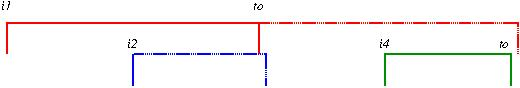
\includegraphics[width=.8\textwidth]{wiggling.jpg}
\end{center}
\caption{A timed behavior with two races}
\label{fig:races}
\end{figure}
\fi
This timed behavior contains two races, after two and four time units, respectively.
The first races is won by block $\{ 1, 3 \}$, and the second race is won by block $\{ 4, 5 \}$.
As a result of these races we cannot wiggle the timing of block $\{ 1, 3 \}$ by any amount:
if $i_1$ occurs just a bit later then timer $y$ must expire before timer $x$,
and if $i_1$ occurs just a bit earlier then timer $u$ must expire before timer $z$.
Note that when timer $x$ expires timer $y$ is stopped.
%
The above scenario is similar to the well-known Rush Hour puzzle game,
in which one has to slide blocking vehicles out of the way to find a path for one specific red car to exit a parking lot.
The next lemma asserts that we can always solve the puzzle for MMTs: for any timed behavior that contains races,
an equivalent timed behavior exists without races.
We may for instance slightly modify the timed behavior
\iflong
of Figure~\ref{fig:races} 
\fi
by scheduling block $\{ 2  \}$
a bit later and block $\{ 4, 5 \}$ a bit earlier.
Then all races have been eliminated and we can wiggle block $\{ 1, 3 \}$.

%We call a valuation $\tvals$ \emph{fraction-injective} if, for all distinct timers $x$ and $y$ in the domain of $\tvals$,
%the fractional parts of $x$ and $y$ are different.
%Note the any fraction-injective valuation is also injective.

\begin{lemma}
\label{race elimination}
Let $\sigma$ be any timed behavior.
Then there exists a timed behavior $\sigma'$ without races such that $\untime(\sigma)=\untime(\sigma')$.
\end{lemma}
\iflong
\begin{proof}
(Sketch) Let
\begin{eqnarray*}
\sigma & = & \tvals_0 \xrightarrow{d_1} \tvals'_0 \xrightarrow{i_1/o_1, \rho_1} \tvals_1 \xrightarrow{d_2} \tvals'_1 \xrightarrow{i_2/o_2, \rho_2} \tvals_2 \cdots
\xrightarrow{d_k} \tvals'_{k-1} \xrightarrow{i_k/o_k, \rho_k} \tvals_{k}.
\end{eqnarray*}
be a timed behavior.
%
For each index $j$, each timer in the domain of $\kappa_j$ has been started by some preceding event.
Let $\startedby_j : \domof{\kappa_j} \rightarrow \Pi_\sigma$ be the function that maps each timer in
the domain of $\kappa_j$ to the block that contains the event that started this timer.
Suppose that $\sigma$ contains a race, that is, there is an index $j>0$ and a timer $x$  
such that $\kappa'_{j-1}(x) = 0$ and $i_j \neq \toevent{x}$.
Let $B \in \Pi_\sigma$ be the block containing $j$. Then we say that block $B$ is the \emph{winner} of the race and block
$\startedby_{j-1}(x)$ is a \emph{loser}.
Note that whenever there is a race at $j$, this race has a single winner but it may have several losers.
Moreover, each block can be loser in at most one race.
A block that does not win any race can be wiggled forward by a small amount (if you don't win you might as well start later).
If block $B$ wins a race from block $B'$, then $\max(B)>\max(B')$, that is, $B$ contains an event that occurs later
in $\sigma$ than any event of $B'$.
This implies that the winning relation induces a partial order on the blocks of $\Pi_\sigma$.
Now consider the bottom elements in this partial order. These blocks do not win any race so we may wiggle them forward.
Once we have eliminated the bottom elements we can work our way upwards in the partial order and wiggle all blocks
forward one by one until no more races remain.
\end{proof}
\fi

%\marginpar{Races are sort of a limit case. I would like to state a corollary here that the set of timed behaviors that contain races have ``measure'' $0$. }

In a timed behavior, there is always an integer amount of time between events from the same block.
This means that, if we consider the absolute time at which events occur, the fractional part of the absolute times
of occurrence is the same for all events in a block.
We call a timed behavior \emph{transparent} if the fractional part of the absolute times of any pair of events from different blocks is different. Note that a transparent timed behavior contains no races.
We call a timed word $w$ \emph{transparent} if there exists a transparent timed behavior $\sigma$ with 
$w = \timedword(\sigma)$.

\begin{lemma}
\label{lemma: transparent timed behavior}
For each feasible untimed behavior $\beta$ there exists
a transparent timed behavior $\sigma$ such that $\beta = \untime(\sigma)$.
\end{lemma}
\iflong
\begin{proof}
Let $\beta$ be a feasible untimed behavior.
Then there exists a timed behavior $\sigma$ such that $\beta = \untime(\sigma)$.
By Lemma~\ref{race elimination}, we may assume that $\sigma$ contains no races.
By repeated application of Lemma~\ref{wiggle lemma}, we can wiggle the timing of all the blocks to make $\sigma$ transparent.
\end{proof}
\fi

Consider a timed word
$w  =   d_1 ~ i_1 ~ o_1 ~ d_2 ~ i_2 ~ o_2 \cdots d_k ~ i_k ~ o_k$.
We want to know, for each timeout event in $w$, by which event this timeout is triggered.
Let $T = \{ j \mid i_j = \mathit{to} \}$ be the set of indices corresponding to a timeout.
A \emph{causality map} for $w$ is a function $c: T \rightarrow \{ 1 ,\ldots, k \}$ that satisfies the following conditions:
\begin{enumerate}
\item
$c$ is injective (at most one timer is started on each transition),
\item
for all $j$, $c(j) < j$ (a timeout is triggered by an earlier event),
\item
for all $j$, $\sum_{l=j+1}^{c(j)} d_l$ is an integer (timers expire after an integer delay).
\end{enumerate}
It is easy to see that a timed word has a causality map iff it is a timed word of an MMT that starts at most one timer
on each transition. In general, a timed word may have multiple causality maps.
However, we have the following lemma.

\begin{lemma}
\label{lemma unique causality map}
A transparent timed word has a unique causality map.
\end{lemma}

Each timed word of MMT $\M$ with a unique causality map has a unique timed run that corresponds to it.
The causality map tells us which timers time out during the trace, so we have complete information
about the sequence of events that occurs. 
\iflong
A timed run of $\M$ is fully determined
by the sequence of time delays and events that occurs.

\begin{lemma}
\label{lemma unique timed run}
Suppose $w$ is a timed word of MMT $\M$ with a unique causality map.
Then there is a unique timed run $\alpha$ of $\M$ such that $w = \timedword(\alpha)$.
\end{lemma}

\fi
We are now prepared to prove our first main result:

\begin{theorem}
\label{timedimpliesuntimed}
Suppose that $\M$ and $\N$ are timer live MMTs in which at most one timer is started on each transition. Then
$\M \approx_{\mathit{timed}} \N$
implies
$\M \approx_{\mathit{untimed}} \N$.
\end{theorem}
\iflong
\begin{proof}
\marginpar{Proof needs doing}
Suppose that $\M \approx_{\mathit{timed}} \N$.
Let $\beta$ be a feasible untimed behavior of $\M$.
By Lemma~\ref{lemma: transparent timed behavior}, there exists a 
a transparent timed behavior $\sigma$ such that $\beta = \untime(\sigma)$.
Let  $w = \timedword(\sigma)$.
Then $w$ is a timed word of $\M$ that has a unique causality map by Lemma~\ref{lemma unique causality map}.
Since $\M \approx_{\mathit{timed}} \N$, $w$ is also a timed word of $\N$.
Let $\alpha$ be the unique (by Lemma~\ref{lemma unique timed run}) timed run such that $w = \timedword(\alpha)$,
and let $\beta' = \untime(\beh(\alpha))$.
Note that the mappings $\timedword$, $\untime$ and $\beh$ all preserve the number of events, the sequence of inputs that occur (except for the names of the timers in timeouts), and the sequence of outputs.

By induction on the number of events in $\beta$ and $\beta'$, we prove that they are isomorphic.
Since $\approx_{\mathit{untimed}}$ is symmetric, this suffices to prove the theorem.

Induction base. If $\beta$ and $\beta'$ contain $0$ events then they are both equal to the empty set of variables $\emptyset$,
and thus trivially isomorphic.

Induction step. Suppose $\beta$ contains $k+1$ events:
\begin{eqnarray*}
\beta & = & X_0 \xrightarrow{i_1/o_1, \rho_1} X_1  \xrightarrow{i_2/o_2, \rho_2} X_2 \cdots \xrightarrow{i_k/o_k, \rho_k} X_{k}
 \xrightarrow{i_{k+1}/o_{k+1}, \rho_{k+1}} X_{k+1}.
\end{eqnarray*}
Let $\delta$ be the prefix of $\beta$ containing $k$ events. Then $\delta$ is also a feasible untimed behavior and thus, by
induction hypothesis, there exists an isomorphism $f = f_0 ,\ldots, f_k$ and a feasible untimed behavior
\begin{eqnarray*}
\delta' & = & Y_0 \xrightarrow{i_1/o_1, \tau_1} Y_1  \xrightarrow{i_2/o_2, \tau_2} Y_2 \cdots \xrightarrow{i_k/o_k, \tau_k} Y_{k}
\end{eqnarray*}
of $\N$ such that $\delta' = f(\delta)$.
\end{proof}
\fi

In the remainder of this article, we only consider timer live MMTs in which at most one timer is started on each transition,
which means we may assume equivalence of the timed and the untimed semantics.

\section{Reachability analysis}
\iflong
It is not difficult to translate an MMTs to a timed automaton \cite{AD94,BengtssonY03} that accepts the same timed words.
Through such a translation, verification and analysis tools for timed automata, such as Uppaal \cite{Uppaal4.0}
become available for MMTs.
MMTs are less expressive than timed automata. MMTs, for instance, do not contain time deadlocks or zeno loops that
may prevent time from progressing.
\fi

MMTs have infinitely (in fact even uncountably) many configurations and it is thus necessary to use symbolic representations
for reachability analysis. Given an untimed behavior $\beta$ we want to compute its effect on a set of valuations. 
If $\beta =X_0$ and $K \subseteq\Vals{X_0}$ then we define $\Post_{\beta}(K) = K$.
If $\beta = X_0 \xrightarrow{i_1/o_1, \rho_1} X_1$ and
$K \subseteq\Vals{X_0}$ then
\begin{eqnarray*}
\Post_{\beta}(K) & = & \{ \tvals'' \in\Vals{X_1} \mid \exists \tvals \in K \exists d >0 \exists \tvals' \in\Vals{X_0} :
 \tvals \xrightarrow{d} \tvals' \xrightarrow{i_1/o_1, \rho_1} \tvals'' \}.
\end{eqnarray*}
The definition of $\Post_{\beta}(K)$ is extended inductively to arbitrary $\beta$ by 
$\Post_{\gamma \cdot \gamma'}(K) = \Post_{\gamma'} (\Post_{\gamma}(K))$, where $\gamma \cdot \gamma'$ is the decomposition of
$\beta$ into an untimed behavior $\gamma$ of length one and an untimed behavior $\gamma'$.
We write $\Post_{\beta}$ as abbreviation for $\Post_{\beta}(\Vals{\Head{\beta}})$.

For any untimed behavior $\beta$, $\Post_{\beta}$ can be symbolically represented and computed using a Difference Bound Matrices (DBMs)
 \cite{Di89},  as the transition relations $\xrightarrow{d}$ and $\xrightarrow{i_1/o_1, \rho_1}$ can be decomposed 
into elementary operations on DBMs such as reset, conjunction, and delay successors \cite{BengtssonY03}.
%
It is easy to see that an untimed behavior $\beta$ is feasible iff $\Post_{\beta} \neq \emptyset$.
Since emptiness of DBMs is decidable, this allows us to compute whether or not $\beta$ is feasible.

\iflong
The next technical lemma's are needed further on:

\begin{lemma}
\label{lemma: feasibility concatenation}
Suppose $\beta, \beta'$ are untimed behaviors with
% $\Last{\beta} = \Last{\beta'} = X_1$ and 
$\Post_{\beta} = Post_{\beta'}$. Let $\gamma$ be any untimed behavior.
Then $\beta \cdot \gamma$ is feasible iff $\beta' \cdot \gamma$ is feasible.
\end{lemma}

\begin{lemma}
\label{lemma finitely many zones}
The set
$\{ \Post_{\beta} \mid \beta \mbox{ is a feasible untimed behavior of } \M \}$ is finite.
\end{lemma}

\begin{proof}
All the sets $\Post_{\beta}$ can be represented using DBMs. Since an MMT only has a finite number of timers that can only be set to a finite number of integer values. Since in an MMT the values of timers can only decrease, only finitely many numbers may
appear in the DBM's that represent the sets $\Post_{\beta}$. Thus all the sets $\Post_{\beta}$ can be represented by a finite
collection of DBMs.
\end{proof}

\begin{lemma}
Suppose $\beta$ is a feasible untimed behavior and $Y \xrightarrow{i/o, \rho} Y'$ is an untimed behavior,
with $Y = \Last{\beta}$ and $i \in I$.
Then $\beta \xrightarrow{i/o, \rho} Y'$ is a feasible untimed behavior.
\end{lemma}

Let $\beta$ be a feasible untimed behavior and let $x \in X$ be a timer. Then we say that $x$ is \emph{expirable} after $\beta$
if there exists a valuation in $\Post_{\beta}$ in which $x$ is minimal.

\begin{lemma}
Suppose $\beta$ is a feasible untimed behavior and $Y \xrightarrow{\toevent{x}/o, \rho} Y'$ is an untimed behavior 
with $Y = \Last{\beta}$.
Then $x$ is expirable after $\beta$ iff $\beta \xrightarrow{\toevent{x}/o, \rho} Y'$ is feasible.
\end{lemma}

\begin{lemma}
\label{not untimed}
Suppose $\M$ and $\N$ are MMTs with $\M \not\approx_{\mathit{untimed}} \N$.
Then there exists a feasible untimed behavior $\beta$ of $\M$ that is not isomorphic to any feasible untimed
behavior of $\N$.
\end{lemma}

\begin{lemma}
\label{not timed}
Suppose $\M$ and $\N$ are MMTs with $\M \not\approx_{\mathit{timed}} \N$.
Then there exists a transparent timed word $w$ of $\M$ that is not a timed word of $\N$.
\end{lemma}

\marginpar{What is the complexity of deciding eg timed equivalence or reachability of MMTs?}
\fi

\section{Learning algorithm}  
In this section, we consider three instances of Angluin's MAT framework.
In the first instance, the teacher knows an MMT $\M$, and the learner poses membership queries
to learn the untimed behaviors of $\M$, and equivalence queries to check whether an hypothesis is correct.
In the second instance, the teacher also knows an MMT $\M$, but now the 
learner performs timed experiments to learn about the
timed words of $\M$, and poses equivalence queries and lookahead queries.
The third instance is the well known setting (see e.g.\ \cite{Nie03,RSBM09}) 
in which the teacher knows an (untimed) Mealy machine $\A$,
and the learner performs membership and equivalence queries.
%
We will show how an untimed teacher for MMTs can be implemented using a timed teacher for MMTs,
and how an untimed learner for MMTs can be implemented using a Mealy machine learner.
%This will allow us to use existing algorithms for learning Mealy machines,
%as implemented for instance in LearnLib \cite{RSBM09}, as part of an algorithm to learn MMTs. 

\subsection{An untimed MAT framework for learning MMTs}
Given the equivalence of the timed and the untimed semantics of MMTs, it is natural to also 
consider an untimed setting, in which a learner tries to construct an MMT based on membership queries for untimed behaviors.
The teacher, however, does not reveal the names of the timers that occur in untimed behaviors, and brings each behavior into a
``canonical'' form, so that a learner can only observe untimed behaviors up to isomorphism.

Let us formalize these ideas.
Suppose $\beta$ be an untimed behavior in which each transition updates at most one timer.
We say that $\beta$ is in \emph{canonical form} if, for each $j$, the timer that is updated in the $j$-th event
(if any) is equal to $x_j$.
For each untimed behavior $\beta$ in which each transition updates at most one timer, there is a unique untimed behavior
$\beta'$ in canonical form that is isomorphic to $\beta$.
We write $\can{\beta}$ to denote this $\beta'$.

An \emph{untimed input word} over $I$ is a sequence $u = i_1 \cdots i_k$ over $\extinputs$ such that (1)
for all indices $j, l$, $i_j = \toevent{x_l}$ implies $l < j$, and (2) each timer occurs at most once in a timeout event.
The first condition  says that if a timer expires it must have been set in a previous event, and the second condition  expresses that
each timer may expire at most once.
Let $\beta$ be an untimed behavior in canonical form.
We can associate a unique input word $\untimedinputword(\beta)$ to $\beta$ by removing all the output events,
updates, and timer sets from $\beta$.

In our first learning setup, the teacher knows an MMT $\M$.
The learner initially knows the set $I$ of inputs of $\M$, and may pose two types of queries:
\begin{itemize}
\item
With a \emph{membership query}, the learner asks for the response to an untimed input word $u$ over $I$.
If $\M$ has a feasible untimed behavior $\beta$ with $\untimedinputword(\can{\beta}) = u$ then the teacher answers
$\can{\beta}$. Otherwise, the answer is $\perp$ (``undefined'').
\item
An \emph{equivalence query} $\CH$, where $\CH$ is an MMT with inputs $I$.
Upon receiving $\CH$, the teacher answers \emph{yes} if $\CH \approx_{\mathit{untimed}} \M$.
Otherwise it answers \emph{no} and supplies a counterexample, that is, a behavior $\beta$ in canonical form that
is isomorphic to a feasible behavior of $\M$ but not to a feasible behavior of $\CH$.
\end{itemize}

\subsection{A timed MAT framework for learning MMTs}
In our second learning setup, the teacher also knows an MMT $\M$.
Initially, the timed learner knows the set $I$ of input of $\M$.
The task of the timed learner is to learn $\M$ through three types of queries: membership queries, equivalence queries,
and lookahead queries.

\paragraph{Membership queries.}
A \emph{timed input word} is a sequence
$u = d_1 ~ i_1 \cdots d_k ~ i_k ~ d_{k+1}$, where $d_j \in \delays$ and $i_j \in I$, for all $1 \leq j \leq k$,
and $d_{k+1} \in \realsplus$.
A timed input word describes an experiment that may be carried out on an MMT. We provide a series of inputs at specific times, and record all the outputs that occur in response to these inputs up to and including the finishing time of the experiment, that is $\sum_{j=1}^{k+1} d_j$.
Since we want to rule out race conditions, we require that the fractional part of the absolute times of occurrence of
all the inputs are different.
Let $w$ be a transparent timed word of $\M$.
We can associate a unique timed input word $\timedinputword(w)$ to $w$ by 
removing all the outputs events, 
removing all occurrences of $\mathit{to}$, 
replacing consecutive numbers by their sum, 
and possibly placing $0$ at the end of the sequence.
Thus, for instance,
\begin{eqnarray*}
\timedinputword (3 ~ i_1 ~ o_1 ~ 1.1 ~ i_2 ~ o_2 ~ 2 ~ \mathit{to} ~ o_3 ~ 2.1 ~ i_4 ~ o_4) & = & 
3 ~ i_1 ~ 1.1 ~ i_2 ~ 4.1 ~ i_4 ~ 0.
\end{eqnarray*}
\iflong
Note that the first input occurs at time $3$, the second at time $4.1$, and the third at time $8.2$.
Thus the fractional part of the times of the inputs are different.
\fi
%
If $u$ and $u'$ are timed input words, then we write $u \propto u'$ if $u$ and $u'$ are equal, except that the final delay of $u$ is less or equal than the final delay of $u'$. Observe that,
for any timed input word $u$ over $I$, 
there exists a unique maximal timed word $w$ of $\M$ such that $\timedinputword(w) \propto u$.
With a \emph{membership query}, the learner asks what the output is in response to a timed input word $u$ over $I$. 
The teacher answers with the unique maximal timed word $w$ of $\M$ such that $\timedinputword(w) \propto u$.

\paragraph{Equivalence queries.}
With an \emph{equivalence query}, the learner asks if a hypothesized MMT $\CH$ is correct, that is, 
whether $\CH \approx_{\mathit{timed}} \M$.
The teacher answers \emph{yes} if this is the case. Otherwise she answers \emph{no} and supplies a
\emph{counterexample}: a transparent timed word $w$ of $\M$ that is not a timed word of $\CH$.
\iflong
(By Lemma~\ref{not timed} 
\else
(We claim that
\fi
such a timed word always exists.)

\paragraph{Lookahead queries.}
A key question that a learner needs to answer is which timers are active after some untimed input word $u$.
Since we assume that there are no ghost variables, a timer that is active after $u$ can expire eventually,
following some further inputs.
In general, however, it may be very difficult to find an input sequence that demonstrates that a timer is active: we may have combination lock scenarios
in which a timer only expires after some very specific, long sequence of inputs.
The search for such a sequence may require an exponential number of membership queries.
However, if when we look at the actual use of timers in protocols, combination lock scenarios just do not occur:
timeouts are not triggered by the occurrence of complicated sequences of inputs, 
but rather by the \emph{absence} of certain inputs.
Simply waiting and providing no inputs at all is usually enough to demonstrate that some timer has been set.
We encapsulate the search for a proof that a timer is active into a \emph{lookahead oracle}:
by posing a \emph{lookahead query}, a timed learner asks if, for some untimed input sequence $u = i_1 \cdots i_k$ and some
index $j \leq k$, timer $x_j$ is active after $u$ in $\M$.
The teacher/oracle answers \emph{yes} if this is the case, and \emph{no} otherwise.

\subsection{A MAT framework for learning Mealy machines}
We will present an algorithm for an untimed learner, by using existing algorithms for learning Mealy machines as a basis.

A \emph{Mealy machine (MM)} is a tuple $\A = (I, O, Q, q_0, \delta, \lambda)$, where
$I$ is a finite set of inputs,
$O$ is a finite set of outputs,
$Q$ is a finite set of states,
$q_0 \in Q$ is the initial state,
$\delta: Q \times I \rightarrow Q$ is a transition function, and
$\lambda: Q \times I \rightarrow O$ is an output function.
%
Output function $\lambda$ is extended to sequences of inputs by defining,
for all $q \in Q$, $i \in I$ and $\sigma \in I^{\ast}$,
%\begin{eqnarray*}
%\delta(q, \epsilon) = q &,~~~ & \delta(q, i \sigma) = \delta(\delta(q,i), \sigma),\\
$\lambda(q, \epsilon) = \epsilon$ and $\lambda(q, i \sigma) = \lambda(q, i) \lambda(\delta(q, i), \sigma)$.
%\end{eqnarray*}
%
The behavior of Mealy machine $\A$ is defined by function $A_\A : I^{\ast} \rightarrow O^{\ast}$ with
$A_\A(\sigma) = \lambda (q^0, \sigma)$, for  $\sigma \in I^{\ast}$.
Mealy machines $\A$ and $\B$ are \emph{equivalent}, denoted $\A \approx \B$, iff $A_{\A} = A_{\B}$.
Sequence $\sigma \in I^{\ast}$ \emph{distinguishes}
$\M$ and $\N$ if and only if $A_{\M}(\sigma) \neq A_{\N}(\sigma)$.

In our third learning setup, the teacher knows a Mealy machine $\M$. 
The learner initially knows the inputs $I$ of $\M$ and may ask two types of queries:
\begin{itemize}
\item
With a \emph{membership query}, the learner asks for the response to an input sequence $\sigma \in I^{\ast}$.
The teacher answers with output sequence $A_{\M}(\sigma)$.
\item
With an \emph{equivalence query}, the learner asks if a hypothesized Mealy machine $\CH$ with
inputs $I$ is correct, that is, whether $\CH$ and $\M$ are equivalent.
The teacher answers \emph{yes} if this is the case. Otherwise she answers \emph{no} and supplies a
\emph{counterexample} $\sigma \in I^{\ast}$ that distinguishes $\CH$ and $\M$.
\end{itemize}
The $L^{\ast}$ algorithm of Angluin \cite{Ang87} is able to learn Mealy machine $\M$ by asking a
number of membership and equivalence queries that polynomial in the size of the corresponding canonical Mealy machine.
Efficient implementations of $L^{\ast}$ and other algorithms for learning Mealy machines are available,
for instance in the tool \learnlib\ \cite{Nie03,RSBM09,MertenSHM11}.

\subsection{Constructing an untimed MMT learner using a MM learner}
The number of timers that may occur in canonical untimed behaviors grows unboundedly with the length of these behavior,
since timers are never reused in canonical behaviors.
Let $S$ be the set of canonical versions of the untimed behaviors of an MMT $\M$.
Then there is a fixed upper bound on the number of timers that are active in a behavior in $S$ at any point,
since $\M$ only has a finite number of timers that it may use.
This means that we can effectively construct a function that maps each untimed behavior $\beta \in S$
to an isomorphic behavior $\uncan{\beta}$ in such a way that only finitely many
different behaviors occur in all the behaviors in the range of $\mathit{uncan}$.
For instance, if a transition occurs in a state in which the set of active timers is $Y$, and this transition
starts a new timer, then $\mathit{uncan}$ may compute the smallest index $j$
such that $x_j \not\in Y$, and then choose $x_j$ as the name of the new timer.
Note that that the timers that occur in $\uncan{S}$ may be different from the timers used by $\M$.

Our algorithm for an untimed learner is based on the following result, which is variant of the famous 
Myhill-Nerode theorem for MMTs.

\begin{definition}
Let $S$ be a set of feasible untimed behaviors over $I$. Then $S$ is
\begin{itemize}
\item
\emph{prefix closed}: $\beta \beta' \in S \Rightarrow \beta \in S$,
\item
\emph{behavior deterministic}:
$\beta \xrightarrow{i/o_1, \rho_1} X_1 \in S \wedge \beta \xrightarrow{i/o_2, \rho_2} X_2 \in S \Rightarrow o_1 = o_2 \wedge \rho_1 = \rho_2 \wedge X_1 = X_2$,
\item
\emph{input complete}:
$\beta \in S \wedge i \in I \Rightarrow \exists o, \rho, Y : \beta \xrightarrow{i/o, \rho} Y \in S$,
\item
\emph{timeout complete}:
$\beta \in S \wedge x \mbox{ expirable after } \beta \Rightarrow
\exists o, \rho, Y: \beta \xrightarrow{\toevent{x}/o, \rho} Y \in S$.
\end{itemize}
Behaviors $\beta, \beta' \in S$ are \emph{equivalent} for $S$, notation $\beta \equiv_S \beta'$, iff 
for any untimed behavior
$\gamma$, $\beta \cdot \gamma \in S \Leftrightarrow \beta' \cdot \gamma \in S$.
We write $[\beta]$ to denote the equivalence class of $\beta$ with respect to $\equiv_S$.
\end{definition}

\begin{theorem}
\label{Nerode theorem}
Let $S$ be a set of feasible untimed behaviors over finite sets of inputs $I$ and outputs $O$.
Then $S$ is the set of feasible untimed behaviors of an MMT $\M$ iff $S$ is nonempty, all untimed behaviors in $S$
start with the empty set of timers, the set of timers that occur in $S$ is finite,
$S$ is prefix closed, behavior deterministic, input complete, timeout complete,
and $\equiv_S$ has only finitely many equivalence classes (finite index).
\end{theorem}
\iflong
\begin{proof}

``$\Rightarrow$'' Let $\M$ be an MMT and let $S$ be the set of its feasible untimed behaviors.
Then it is immediate from the definitions that $S$ is nonempty, all untimed behaviors in $S$
start with the empty set of timers, the set if timers that occurs in $S$ is finite,
$S$ is prefix closed, behavior deterministic, input complete, and timeout complete.
Suppose that feasible untimed behaviors $\beta$ and $\beta'$ lead to the same state $q$ and moreover $\Post_{\beta} = \Post_{\beta'}$.
Then, 
by Lemma~\ref{lemma: feasibility concatenation},
for any untimed behavior $\gamma$, $\beta \cdot \gamma \in S \Leftrightarrow \beta' \cdot \gamma \in S$, and thus
$\beta \equiv_S \beta'$.
Since $\M$ only has finitely many states and by Lemma~\ref{lemma finitely many zones} the set
$\{ \Post_{\beta} \mid \beta \mbox{ is a feasible untimed behavior of } \M \}$ is finite, this means that
$\equiv_S$ has finite index.

``$\Leftarrow$'' Suppose $S$ is nonempty, etc.
Let MMT $\M = (I, O \cup \{ \perp \}, Q, q_0, \vars, \delta, \lambda, \remap)$ be defined as follows:
\begin{itemize}
\item
$\perp$ is a special, fresh output event.
\item
$Q$ is the set of equivalence classes of $\equiv_S$.
\item
$q_0 = [\emptyset]$. (Note that $\emptyset \in S$ since $S$ is nonempty, prefix closed, and all untimed behaviors in $S$ start
with the empty set of timers.)
\item
$\varsof{[\beta]} = \Last{\beta}$.
\item
Let $\beta \in S$ and $i \in I$. Then, since $S$ is both input complete and behavior deterministic, there exist unique
$o$, $\rho$ and $Y$ such that $\beta' = \beta \xrightarrow{i/o, \rho} Y \in S$.
We define $\delta([\beta],i) = [\beta']$, $\lambda([\beta],i) = o$, and $\remap([\beta],i) = \rho$.
\item
Assume $\beta \in S$ and $x\in \Last{\beta}$ expirable after $\beta$. 
Then, since $S$ is both timeout complete and behavior deterministic, there exist unique
$o$, $\rho$ and $Y$ such that $\beta' = \beta \xrightarrow{\toevent{x}/o, \rho} Y \in S$.
We define $\delta([\beta],\toevent{x}) = [\beta']$, $\lambda([\beta],\toevent{x}) = o$, and $\remap([\beta],\toevent{x}) = \rho$.
\item
Assume $\beta \in S$ and $x \in \Last{\beta}$ not expirable after $\beta$.
We define $\delta([\beta],\toevent{x}) = [\beta]$, $\lambda([\beta],\toevent{x}) = \perp$, and $\remap([\beta],\toevent{x}) = \rho_0$, where $\domof{\rho_0} = \emptyset$.
\end{itemize}
It is routine to verify that $\M$ is a well-defined MMT whose set of feasible untimed behaviors equals $S$.
\end{proof}
\fi

The canonical MMT $\M$ constructed in the proof of Theorem~\ref{Nerode theorem} has a special property: an untimed
behavior of $\M$ is feasible iff it does not contain
\iflong
the
\else
a
\fi
special output event $\perp$. Call an MMT that satisfies this property
\emph{transparent}. 
We say that a timer $x$ \emph{may expire} in a state $q$ if $q$ has an outgoing $\toevent{x}$ transition with
an output different from $\perp$.
In a transparent MMT, a timer may expire after an untimed behavior $\beta$ iff it may expire in the
unique state of $\M$ that is reached by $\beta$.
%
Note that, for any MMT $\N$ there exists an equivalent transparent MMT $\M$, since
from the set $S$ of feasible untimed behaviors of $\N$ we may construct an equivalent transparent MMT using the construction
of Theorem~\ref{Nerode theorem}.
Our learning algorithm requires a number of queries that is polynomial in the size of the minimal transparent MMT that is equivalent to the given MMT.

Our algorithm for an untimed learner now looks as follows.
\marginpar{Needs doing}

%Let $\M = (I, O, Q, q_0, \vars, \delta, \lambda, \remap)$ be a transparent MMT with $\perp \in O$.
%Let $Y = \bigcup_{q \in Q} \varsof{q}$ be the set of timers that appear in $\M$.
%We associate to $\M$ a Mealy machine $\Mealy(\M) = (I', O', Q, q_0, \delta', \lambda')$ where
%\begin{itemize}
%\item
%$I' = I \cup \{ \toevent{x} \mid x \in Y \}$
%\item
%$O' = O \times (X \hookrightarrow \natplus)$
%\item
%$\delta'(q,i) = \left\{ \begin{array}{ll}
%\delta(q,i) & \mbox{if } i \in I \mbox{ or } \exists x \in \varsof{q} : i = \toevent{x} \mbox{ and } \lambda(q,i) \neq \perp\\
%q & \mbox{otherwise}
%\end{array} \right.$
%\item
%$\lambda'(q,i) = \left\{ \begin{array}{ll}
%(\lambda(q,i), \rho(q,i), \varsof{q}) & \mbox{if } i \in I \mbox{ or } \exists x \in \varsof{q} : i = \toevent{x} \mbox{ and } \lambda(q,i) \neq \perp\\
%(\perp,\emptyset) & \exists x \in \varsof{q} : i = \toevent{x} \mbox{ and } \lambda(q,i) = \perp\\
%(\ast,\emptyset) & \mbox{otherwise}
%\end{array} \right.$
%\end{itemize}
%
%\begin{theorem}
%\label{untimedequivalentmealy}
%Let $\M$ and $\N$ be transparent MMTs.
%Then $\M \approx_{\mathit{untimed}} \N$
%iff
%$\Mealy(\M) \approx \Mealy(\N)$.
%\end{theorem}

\subsection{Constructing an untimed MMT teacher using a timed teacher}
In this subsection, we show how we may construct a teacher for the untimed setting, while using the
teacher for the timed setting.

Suppose the untimed teacher receives a membership query, consisting of an untimed input word
$u = i_1 \cdots i_k$.
Inductively, we construct a response for $u$ by the untimed teacher.
If $k=0$, then we take $\beta = \emptyset$.
This is an untimed feasible behavior of $\M$ in canonical form with $\untimedinputword(\beta)=u$.
For the induction step, suppose that $k>0$.
If the computed answer for $i_1 \cdots i_{k-1}$ is $\perp$, then the answer for $u$ is also $\perp$.
Otherwise, let $\beta$ be the computed answer for $i_1 \cdots i_{k-1}$.
Then $\beta$ is the canonical form of a feasible untimed behavior of $M$, and $\untimedinputword(\beta)=u$.
Let $Y$ be the final set of variables of $\beta$.
If $i_k = \toevent{x}$ for some timer $x$ that is not expirable after $\beta$ then there exists no feasible behavior
with untimed input word $u$. In this case, the untimed teacher may return the answer $\perp$.
Otherwise  Etc etc
\marginpar{Needs doing}

Once we have implemented membership queries for an untimed teacher, implementing equivalence queries is easy.
Suppose that the untimed teacher receives an equivalence query $\CH$.
Then we just forward this query to the timed teacher.
If the timed teacher answers \emph{yes} then $\CH \approx_{\mathit{timed}} \M$.
In this case, by Theorem~\ref{timedimpliesuntimed}, $\CH \approx_{\mathit{untimed}} \M$,
and thus the untimed teacher can also return a result \emph{yes}.
If the timed teacher answers \emph{no} and returns a counterexample $w$,
then $w$ is a transparent timed word of $\M$ but not of $\CH$.
In this case, by Theorem~\ref{untimedimpliestimed}, we may conclude that
$\CH \not\approx_{\mathit{untimed}} \M$, and thus the untimed teacher can also return a result \emph{no}.
Since $w$ is a transparent timed word of $\M$, it follows by Lemma~\ref{lemma unique causality map}
that $w$ has a unique causality map $c$.
This allows us to transform $w$ into an untimed input sequence $u$: 
we remove all the delays and output events, and if the $j$-th
input in $w$ equals $\mathit{to}$, we replace it by $\toevent{x_{c(j)}}$.
We perform an untimed membership query for $u$, and let the untimed teacher return the resulting 
untimed behavior $\beta$ as counterexample.






